% Adapted from LaTeX-examples-master/tikz/triangle-inscribed-circle.
% Exercises the native tkz-euclide [in] circle and three internal bisectors.
\documentclass[border=3pt]{standalone}
\usepackage{tikz}
\usepackage{tkz-euclide}

\begin{document}
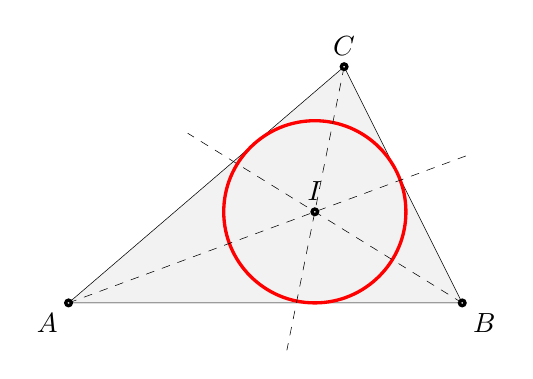
\begin{tikzpicture}[very thick]
  \tkzDefPoints{0/0/A,5/0/B,3.5/3/C}
  \tkzDrawPolygon[fill=gray!10](A,B,C)

  \tkzDefCircle[in,/tikz/overlay](A,B,C)\tkzGetPoints{I}{T}
  \tkzDrawCircle[color=red,very thick](I,T)

  \tkzDefLine[bisector,/tikz/overlay](B,A,C)\tkzGetPoint{a}
  \tkzInterLL(A,a)(B,C)\tkzGetPoint{a2}
  \tkzDrawLine[add=0 and 0.2,dashed](A,a2)

  \tkzDefLine[bisector,/tikz/overlay](A,C,B)\tkzGetPoint{c}
  \tkzInterLL(C,c)(A,B)\tkzGetPoint{c2}
  \tkzDrawLine[add=0 and 0.2,dashed](C,c2)

  \tkzDefLine[bisector,/tikz/overlay](C,B,A)\tkzGetPoint{b}
  \tkzInterLL(B,b)(A,C)\tkzGetPoint{b2}
  \tkzDrawLine[add=0 and 0.2,dashed](B,b2)

  \tkzDrawPoints(A,B,C,I)
  \tkzLabelPoints[below left](A)
  \tkzLabelPoints[below right](B)
  \tkzLabelPoints[above](C)
  \tkzLabelPoint[above](I){$I$}
\end{tikzpicture}
\end{document}
